\documentclass[a4paper]{article}

\usepackage[english]{babel}
\usepackage{amsmath}
\usepackage{color}
\usepackage{amssymb}
\usepackage{dsfont}
\usepackage{multicol}
%\usepackage[lofdepth,lotdepth]{subfig}  This gives errors when used together with "subcaption", which is needed to create subfigures.
\usepackage{graphicx}
\usepackage{listings}
\usepackage[hyphens]{url}
\usepackage{pgf, tikz}
\usetikzlibrary{arrows, automata}
\usepackage{titling}
\usepackage{varwidth}
\usepackage{hyperref}
\usepackage{color} %red, green, blue, yellow, cyan, magenta, black, white
\definecolor{mygreen}{RGB}{28,172,0} % color values Red, Green, Blue
\definecolor{mylilas}{RGB}{170,55,241}
\setlength\parindent{0pt}
\usepackage{float}
\usepackage{subcaption}
\usepackage{polynom}
\usepackage{physics}
\newcommand\tab[1][1cm]{\hspace*{#1}}


\newcommand\independent{\protect\mathpalette{\protect\independenT}{\perp}}
\def\independenT#1#2{\mathrel{\rlap{$#1#2$}\mkern2mu{#1#2}}}

\usepackage{geometry}
 \geometry{
 a4paper,
 total={165mm,257mm},
 left=20mm,
 top=20mm,
 }

\definecolor{codegreen}{rgb}{0,0.6,0}
\definecolor{codegray}{rgb}{0.5,0.5,0.5}
\definecolor{codepurple}{rgb}{0.58,0,0.82}
\definecolor{backcolour}{rgb}{0.95,0.95,0.92}

\lstdefinestyle{mystyle}{
    backgroundcolor=\color{backcolour},   
    commentstyle=\color{codegreen},
    keywordstyle=\color{magenta},
    numberstyle=\tiny\color{codegray},
    stringstyle=\color{codepurple},
    basicstyle=\footnotesize,
    breakatwhitespace=false,         
    breaklines=true,                 
    captionpos=b,                    
    keepspaces=true,                 
    numbers=left,                    
    numbersep=5pt,                  
    showspaces=false,                
    showstringspaces=false,
    showtabs=false,                  
    tabsize=2
}
 
\lstset{style=mystyle}


\DeclareMathOperator*{\argmax}{arg\,max}
\DeclareMathOperator*{\argmin}{arg\,min}

\title{Statistical Machine Learning 2018\\Assignment 4\\Deadline: 11th of January 2019}
\author{
  Christoph Schmidl\\ s4226887\\      \texttt{c.schmidl@student.ru.nl}
  \and
  Mark Beijer\\ s4354834\\     \texttt{mbeijer@science.ru.nl}
}
\date{\today}

\begin{document}
\maketitle


\section*{Exercise 1 - Logistic regression (weight 5)}

\textbf{Part 1 - The IRLS algorithm}\\

Many machine learning problems require minimizing / maximizing some function $f(x)$. For this, an alternative to the familiar gradient descent technique, is the so called Newton-Raphson iterative method:

\begin{eqnarray} \label{eq:1}
\textbf{x}^{(n+1)} = \textbf{x}^{(n)} - \textbf{H}^{-1} \nabla f(\textbf{x}^{(n)})
\end{eqnarray}

where \textbf{H} represents the Hessian matrix of second derivatives of $f(\textbf{x})$, see Bishop, §4.3.3.

\subsection*{1.1.1}

Derive an expression for the minimization / maximization of the function $f(x) = \sin(x)$, using the Newton-Raphson iterative optimization scheme (\ref{eq:1}), and verify (using Matlab, just up to, e.g., five iterations) how quickly it converges when starting from $x^{(0)} = 1$. What happens when you start from $x^{(0)} = -1$?\\
Hint: The Hessian of a 1-dimensional function $f(x)$ is just the second derivative $f''$. So, the Newton-Raphson iterative method reduces in 1-d to 

\begin{eqnarray}  \label{eq:2}
x^{(n+1)} = x^{(n)} - \frac{f'(x^{(n)})}{f''(x^{(n)})}
\end{eqnarray}


\textbf{Answer:}\\

Expression for the minimization / maximization of the function $f(x) = \sin(x)$:

\begin{align*}
x^{(x+1)} &= x^{(n)} - \frac{\sin'(x^{(n)})}{\sin''(x^{(n)})}\\
&=  x^{(n)} - \frac{\cos(x^{(n)})}{-\sin(x^{(n)})}\\
&=  x^{(n)} + \frac{\cos(x^{(n)})}{\sin(x^{(n)})}\\
\end{align*}

\begin{lstlisting}[language=Python]
import numpy as np
import sympy as sp

# Exercise 1.1.1

## See also: https://docs.sympy.org/latest/tutorial/calculus.html

def f(x):
    return np.sin(x)

def iterative_optimization(x):
    """ Using Newton-Raphson iterative optimization scheme """
    return x + (np.cos(x)/np.sin(x))

x_t = 1
n_iterations = 5

print("Starting the optimization process with x_0: {}".format(x_t))

for i in range(n_iterations):
    x_t = iterative_optimization(x_t)
    print("Step {}: {}".format(i, x_t))
    
# Starting the optimization process with x_0: 1
# Step 0: 1.6420926159343308
# Step 1: 1.5706752771612507
# Step 2: 1.5707963267954879
# Step 3: 1.5707963267948966
# Step 4: 1.5707963267948966

# Starting the optimization process with x_0: -1
# Step 0: -1.6420926159343308
# Step 1: -1.5706752771612507
# Step 2: -1.5707963267954879
# Step 3: -1.5707963267948966
# Step 4: -1.5707963267948966
\end{lstlisting}



If we take $x_0 = 1$, then the algorithm converges after 4 steps towards $1.5707963267948966$ which is an approximation of $\frac{\pi}{2}$.\\ 
If we take $x_0 = -1$, then the algorithm converges after 4 steps towards $-1.5707963267948966$ which is an approximation of $-\frac{\pi}{2}$.

\begin{figure}[H]
\center
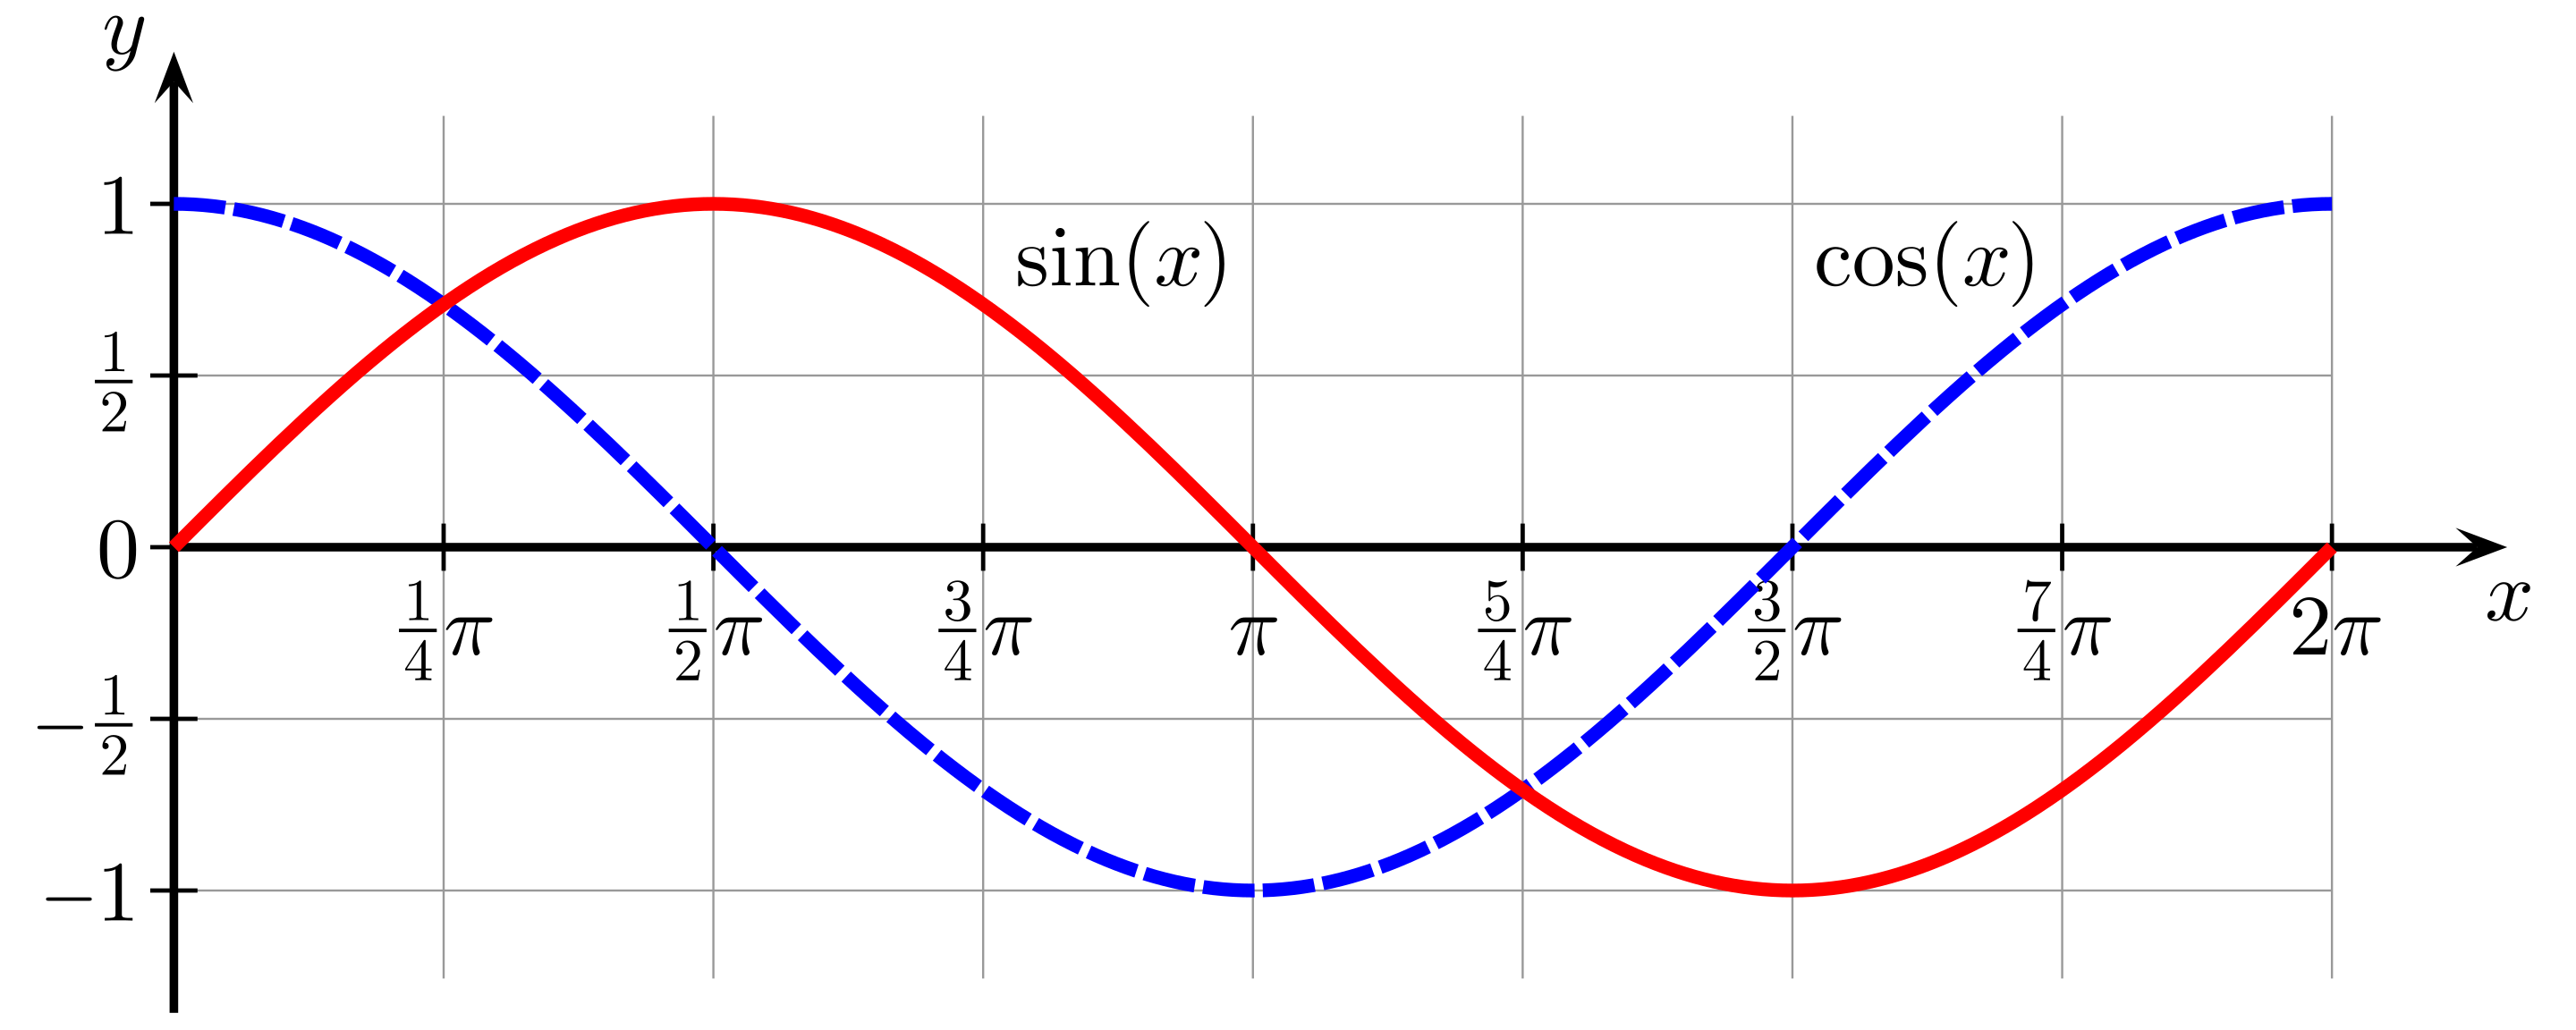
\includegraphics[width=0.6\textwidth]{Images/sine_cosine.png}
\caption{Sine and Cosine}
\label{Fig:sine-cosine}
\end{figure}

When we take a look at figure \ref{Fig:sine-cosine} then we can see that the maximum and minimum of the sine function is indeed at $(x = \frac{\pi}{2}, f(x) = 1)$ and $(x = -\frac{\pi}{2}, f(x) = -1)$ with possible shiftings to the right and left based on the periodic nature of the sine function.\\

Note: Also see \url{https://en.wikipedia.org/wiki/Newton%27s_method#Applications}


\subsection*{1.1.2}


We want to apply this method to the logistic regression model for classification (see Bishop, §4.3.2):

\begin{equation}  \label{eq:3}
p(\mathcal{C}_1 | \phi ) = y(\phi) = \sigma(w^T \phi)
\end{equation}

For a data set $\{ \phi_n, t_n\}^N_{n=1}$, with $t_n \in \{ 0,1 \}$, using $y_n = p(\mathcal{C}_1 | \phi_n)$ the corresponding cross entropy error function to minimize is 

\begin{equation}  \label{eq:4}
E(\textbf{w}) = - \sum^N_{n=1} \{ t_n \ln y_n + (1 - t_n) \ln(1 - y_n)\}
\end{equation}

With one basis function $\phi$ and the dummy basis function 1, the feature vector in (\ref{eq:3}) becomes $\phi = [1, \phi]^T$. The weight vector including the bias term is then also two dimensional, $\textbf{w} = [w_0,w_1]^T$.
Expressions for the gradient $\nabla E(\textbf{w})$ and Hessian \textbf{H} in terms of the data set are given in Bishop, eq.4.96-98. As both are implicitly dependent on the weights \textbf{w}, they have to be recalculated after each step: hence this is known as the 'Iterative Reweighted Least Squares' algorithm.\\

Consider the following data set: $\{ \phi_1, t_1 \} = \{0.3, 1 \}, \{ \phi_2, t_2 \} = \{ 0.44, 0 \}, \{ \phi_3, t_3 \} = \{ 0.46, 1 \}$ and $\{ \phi_4, t_4 \} = \{ 0.6, 0 \}$, and initial weight vector $\textbf{w}^{(0)} = [1.0, 1.0]^T$.\\

Show using e.g. a Matlab implementation that for this situation the IRLS algorithm converges in a few iterations to the optimal solution $\hat{\textbf{w}}^T \approx [9.8, -21.7]$, and show that this solution corresponding to a decision boundary $\phi = 0.45$ in the logistic regression model. (The IRLS algorithm should take about five lines of Matlab code inside a loop + initialization).\\


\textbf{Answer:}\\

\begin{align*}
p(\mathcal{C}_1 | \phi ) = y(\phi) = \sigma(w^T \phi) = \frac{1}{1 + \exp(-(w^T\phi))}
\end{align*}

As stated in Bishop, page 208, eq 4.99 and 4.100: The Newton-Raphson update formula for the logistic regression model becomes 

\begin{align*}
\textbf{w}^{new} &= \textbf{w}^{old} - (\boldsymbol{\Phi} ^T \textbf{R} \boldsymbol{\Phi} )^{-1} \boldsymbol{\Phi} ^T (\textbf{y} - \textbf{t})\\
&= (\boldsymbol{\Phi}^T \textbf{R} \boldsymbol{\Phi} )^{-1} \{ \boldsymbol{\Phi}^T \textbf{R}  \boldsymbol{\Phi} \textbf{w}^{(old)} - \boldsymbol{\Phi}^T (\textbf{y} - \textbf{t})  \}\\
&= (\boldsymbol{\Phi}^T \textbf{R} \boldsymbol{\Phi} )^{-1} \boldsymbol{\Phi}^T \textbf{R} \textbf{z} 
\end{align*}

where \textbf{z} is an N-dimensional vector with elements

\begin{align*}
\textbf{z} = \boldsymbol{\Phi} \textbf{w}^{old} - \textbf{R}^{-1} (\textbf{y} -\textbf{t})
\end{align*}



The following Python code converges after 6 iterations towards $\hat{\textbf{w}}^T = [  9.78227684, -21.73839298]$ which is pretty close to the optimal solution.


\begin{lstlisting}[language=Python]
# Exercise 1.1.2

def sigmoid(x):
    """ The standard logistic function. np.exp also accepts arrays"""
    return 1.0 / (1 + np.exp(-x))

def gradient_of_error(phi, y, t):
    """ Gradient (first-order derivatives) of the error function, see Bishop page 207, eq. 4.96 """
    return np.dot(phi.T, y - t)

def hessian_of_error(phi, y):
    """ Hessian (second-order derivatives) of the error function, see Bishop page 207, eq. 4.97 """
    R = np.diag(np.ravel(y * (1 - y)))
    return np.dot(phi.T, np.dot(R, phi))


w = np.array([ [1.0], [1.0] ]) # two-dimensional weight vector
x = np.array([0.3, 0.44, 0.46, 0.6])
t = np.array([ [1], [0], [1], [0] ]) # targets
phi = np.array([ [1, x_element] for x_element in x ]) # feature vector

for i in range(10):
    y = sigmoid(np.dot(phi, w)) # class estimates
    
    current_gradient = gradient_of_error(phi, y, t)
    current_hessian = hessian_of_error(phi, y)
    
    w = w - np.dot(np.linalg.inv(current_hessian), current_gradient)
    
    print("Iteration {}: \nphi={} \ny={}, \ncurrent_gradient={}, \ncurrent_hessian={}, \nw={}\n".format(
        i, phi, y, current_gradient, current_hessian, w))
    
# Converges after 6 iterations  
# w=[[  9.78227684][-21.73839298]]
\end{lstlisting}

\vspace{1em}

In order to show that $\phi = 0.45$ is indeed the decision boundary, we  show that the probability of a data point with $\phi = 0.45$ is the same for both classes. That means that both classes have a probability of  $0.5$ since $p(C_1 \vert \phi) + p(C_2 \vert \phi) = 1$.

		\begin{align*}
			p(C_1 \vert \phi) = y(\phi) = \sigma (\boldsymbol w^T \phi) = \sigma (\begin{pmatrix} 9.78227684 \\ -21.73839298 \end{pmatrix}^T \begin{pmatrix} 1\\0.45 \end{pmatrix}) \approx 0.50
		\end{align*}

We can also prove that in a slightly different way using the optimal solution:

\begin{align*}
p(C_1 | \phi) &= \frac{1}{1 + \exp(-w^T \phi)}\\
0.5 &= \frac{1}{1 + \exp(-[9.8, -21.7]^T [1, \phi])}\\
0.5 &= \frac{1}{1 + \exp(-9.8 + 21.7 \phi)}\\
2 &= 1 + \exp{-9.8 + 21.7 \phi}\\
1 &= \exp(-9.8 + 21.7 \phi)\\
\ln(1) &= -9.8 + 21.7 \phi\\
0 &= -9.8 + 21.7 \phi\\
21.7 \phi &= 9.8\\
\phi &= \frac{9.8}{21.7} \approx 0.45
\end{align*}


Useful internet resources which helped solving this exercise:

\begin{itemize}
	\item Second Order Optimization - The Math of Intelligence 2: \url{https://www.youtube.com/watch?v=UIFMLK2nj_w}
	\item Logistic Regression - The Math of Intelligence (Week 2): \url{https://www.youtube.com/watch?v=D8alok2P468}
	\item \url{https://thelaziestprogrammer.com/sharrington/math-of-machine-learning/solving-logreg-newtons-method}
	\item \url{http://cs229.stanford.edu/notes/cs229-notes1.pdf}
	\item \url{https://www.stat.cmu.edu/~cshalizi/350/lectures/26/lecture-26.pdf}
	\item \url{https://www.stat.cmu.edu/~cshalizi/402/lectures/14-logistic-regression/lecture-14.pdf}
	\item \url{https://www.khanacademy.org/math/multivariable-calculus/applications-of-multivariable-derivatives/quadratic-approximations/a/the-hessian}
	\item \url{https://web.stanford.edu/group/sisl/k12/optimization/#!index.md}
	\item \url{http://openclassroom.stanford.edu/MainFolder/DocumentPage.php?course=MachineLearning&doc=exercises/ex4/ex4.html}
\end{itemize}




\textbf{Part 2 - Two-class classification using logistic regression}\\

\begin{figure}[H]
\center
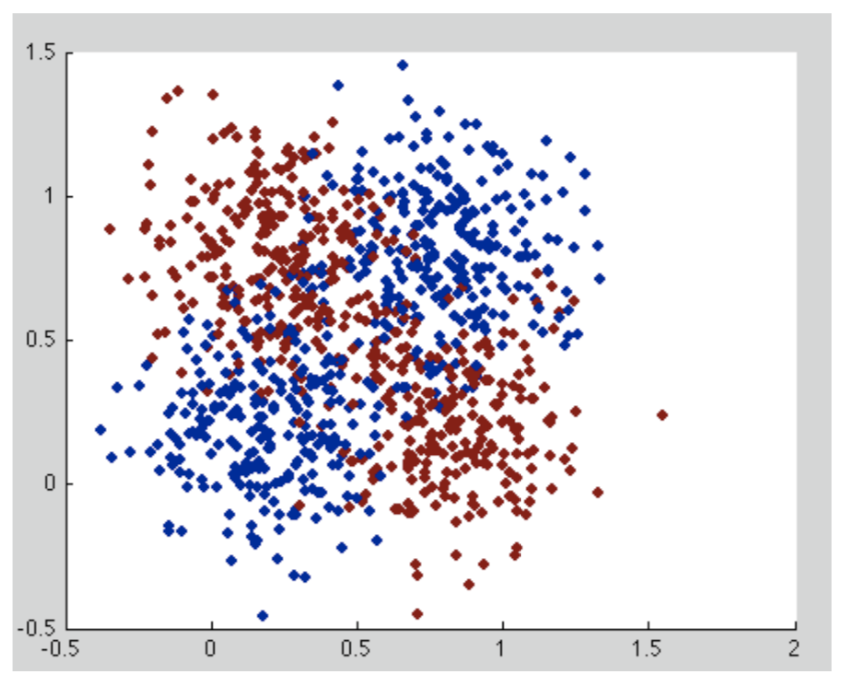
\includegraphics[width=0.4\textwidth]{Images/two-class-dataset.png}
\caption{Two class data for logistic regression}
\label{Fig:two-class-dataset}
\end{figure}

Two-class classification using logistic regression in the IRLS algorith,. Data consists of 1000 pairs $\{ x_1, x_2 \}$ with corresponding class labels $\mathcal{C}_1 = 0$ or $\mathcal{C}_2 = 1$. Load it into Matlab using\\

\hspace{1cm} \texttt{data = load('a010\_irlsdata.txt', '-ASCII');}

\hspace{1cm} \texttt{X = data(:,1:2); Y = data(:,3);}\\

\subsection*{1.2.1}

Make a scatter plot of the data, similar to Figure \ref{Fig:two-class-dataset}. (Have a look at Matlab file \texttt{a010plotideas.m} in Brightspace for some ideas to make such a scatter plot and the plots later on.) Do you think logistic regression can be a good approach to classification for this type of data? Explain why.\\

\textbf{Answer:}\\

The following Python code generates figure \ref{Fig:1_2_1}:

\begin{lstlisting}[language=Python]
# Exercise 1.2.1

data = np.loadtxt("data/a010_irlsdata.txt")

print("Shape of loaded data: {}".format(data.shape))
X = data[:,0:2] # feature vector
print("Shape of feature vector: {}".format(X.shape))

Y = data[:,2:3] # label vector
print("Shape of label vector: {}".format(Y.shape))

# Plot
plt.scatter(X[:,0], X[:,1], c=Y.ravel())
plt.xlabel('X')
plt.ylabel('Y')
plt.savefig('figure_1_2_1.png')
plt.show()
\end{lstlisting}

\vspace{1em}

We do not think that Logistic Regression is a good approach to classify this type of data because the data does not seem to be linearly separable.

The decision boundary drawn by Logistic regression is a linear combination of features and weights denoted by $w_0 + \sum_i w_iX_i$ and therefore is only able to draw a hyperplane through the space to predict one class of each side respectively. The presented data cannot be divided by such a plane except when it would be possible to apply kernel methods like in Support Vector Machines which maps the problem into a new space.\\

See also: \url{https://homes.cs.washington.edu/~marcotcr/blog/linear-classifiers/}


\begin{figure}[H]
\center
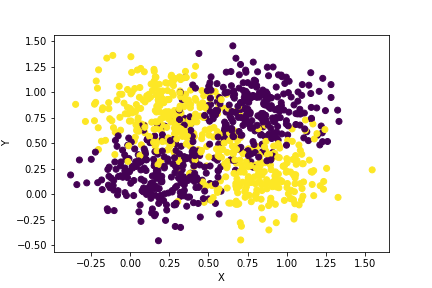
\includegraphics[width=0.6\textwidth]{Images/figure_1_2_1.png}
\caption{Scatter plot of two class data of exercise 1 - Part 2}
\label{Fig:1_2_1}
\end{figure}





\subsection*{1.2.2}

Modify the Iterative Reweighted Least Squares algorithm from part 1 to calculate the optimal weights for this data. Use again a dummy basis function. Initialize with the weight vector $\textbf{w}^T = [0, 0, 0]$. With these initial weights, what are the class probabilities according to the logistic regression model (i.e., before optimization)?\\

\textbf{Answer:}\\








\subsection*{1.2.3}

Run the algorithm. Make a scatter plot of the data, similar to figure \ref{Fig:two-class-dataset}, but now with color that represent the data point probabilities $P(C = 1, X_n)$ according to the model after optimization. Compare the cross entropy error with the initial value. Did it improve? Much? Explain your findings.\\

\textbf{Answer:}\\







\subsection*{1.2.4}

Introduce two Gaussian basis functions as features $\phi_1, \phi_2$, similar to Bishop, fig.4.12. Use identical isotropic covariance matrices $\Sigma = \sigma^2 I$ with $\sigma^2 = 0.2$, and center the basis functions around $\mu_1 = (0,0)$ and $\mu_2 = (1,1)$. Make a scatter plot of the data in the feature domain. Do you think logistic regression can be a good approach to classification with these features? Explain why.\\

\textbf{Answer:}\\










\subsection*{1.2.5}

Modify the IRLS algorithm to use the features $\{ \phi_1, \phi_2 \}$ and the dummy basis function. Initialize with the weight vector $\textbf{w}^T = [0,0,0]$.\\
Run the algorithm. Make a scatter plot of the data, similar to Figure \ref{Fig:two-class-dataset}, but now with colors that represent the data point probabilities $P(C = 1 | X_n)$ according to this second model (after optimization). Compare the cross entropy error with the initial value. Did it improve? Much? Explain your findings.\\


\textbf{Answer:}\\


\section*{Exercise 2 - Neural network regression (weight 5)}

We train a neural network using backpropagation, to learn to mimic a 2D multimodal probability density. First, we implement the network and test its regression capabilities on a standard Gaussian; then we train it on the real data set. Visualization of the network output plays an important role in monitoring the progress.

\subsection*{2.1}

Create a plot of an isotropic 2D Gaussian $y = 3 \cdot \mathcal{N}(\textbf{0}|\frac{2}{5}\textbf{I}_2)$ centered at the origin using the \texttt{meshgrid()}, \texttt{mvnpdf()} and \texttt{surf()} functions. Sample the density at 0.1 intervals over the range $[-2,2] \times [-2,2]$ and store the data in colum vector variables $\textbf{X}$ (2D) and $\textbf{Y}$ (1D).\\

\textbf{Answer:}\\


This can be done by using the following code:

\begin{lstlisting}[language=Python]
def Gaus(X):
    FirstPart = 1/np.power(2*np.pi,len(X)/2)*1/(np.power(np.linalg.det(Sigma),0.5))
    Exp = -(1/2)*np.matmul(np.transpose(X-Mu),np.matmul(np.linalg.inv(Sigma),X-Mu))
    return FirstPart*np.exp(Exp)

def Plot(X,Y,Name):
    x,y = np.hsplit(X,2)
    x = np.reshape(x,(41,41))
    y = np.reshape(y,(41,41))
    z = np.reshape(Y,(41,41))
    fig = plt.figure(Name)
    ax = fig.gca(projection='3d')
    surf = ax.plot_surface(x, y, z, cmap=cm.coolwarm,
                       linewidth=1, antialiased=True)
Sigma = (2/5)*np.identity(2)
Mu = np.zeros(2)
x = y = np.arange(-2,2+0.1,0.1)
x,y = np.meshgrid(x,y)
X = []
for i in range(len(x)):
    for j in range(len(x[0])):
        X.append(np.array([x[i][j],y[i][j]]))
X = np.array(X)
Y = np.array([Gaus(x) for x in X])
\end{lstlisting}

The function "Gaus"(line 1) simply follows the definition of the multi-variable Gaussian as given at page 78 of Bishop.:

\begin{equation}
\mathcal N (x|\mu,\sigma^2) = \frac{1}{(2\pi)^{\frac{D}{2}}} \frac{1}{\abs{\Sigma}^{\frac{1}{2}}} e^{-\frac{1}{2}(x-\mu)^T\Sigma^{-1} (x-\mu)}
\end{equation}

For plotting, we need to reshape it because this is the way that matplotlib plots, it takes 2 2D arrays for X and Y and 1 2D array for z.
The construction with the for-loop ensures that X contains all points required uniquely.
The plot of the Gaussian can be seen at figure \ref{GausPlot}:

\begin{figure}[H]
\includegraphics[width=\textwidth]{Images/Plot_Gaussian.png}
\caption{Gaussian function $Y = 3 \cdot \mathcal{N}(\textbf{0}|\frac{2}{5}\textbf{I}_2)$ graphed.}
\label{GausPlot}
\end{figure}


\subsection*{2.2}

Implement a 2-layer neural network with $D = 2$ input nodes, $K = 1$ output nodes and $M$ hidden nodes in the intermediate layer that can be trained using a sequential error backpropagation procedure, as described in Bishop §5.3. Use $tanh(\cdot)$ activation functions for the hidden nodes and a linear activation function (regression) for the output node. Introduce appropriate weights and biases, and set the learning rate parameter $\eta = 0.1$. Initialize the weights to random values in the interval $[-0.5,0.5]$. Plot a 2D graph of the initial output of the network over the same $[-2,2] \times [-2,2]$ grid as the Gaussian (again using \texttt{surf()}).\\

\textbf{Answer:}\\









\subsection*{2.3}

Train the network for $M = 8$ hidden nodes on the previously stored $\textbf{X}$ and $\textbf{Y}$ values (the $\{ x_1, x_2 \}$ input coordinates and corresponding output probability density $y$), by repeatedly looping over all datapoints and updating the weights in the network after each point. Repeat for at least 500 complete training cycles and monitor the progress of the training by plotting the output of the network over the $\textbf{X}$ grid after each full cycle. Verify the output starts to resemble the Gaussian density after some 200 cycles (all be it with lots of 'wobbles').\\


\textbf{Answer:}\\







\subsection*{2.4}

Permute the $\textbf{X}$ and $\textbf{Y}$ arrays to a random order using the \texttt{randperm()} function, keeping corresponding $x$ and $y$ together. Repeat the network training session using this randomized data set. Verify that convergence is now much quicker. Can you understand why? Try out the effect of different numbers of hidden nodes, different initial weights and different learning rates on speed and quality of the network training. Explain your results.

\begin{figure}[H]
\center
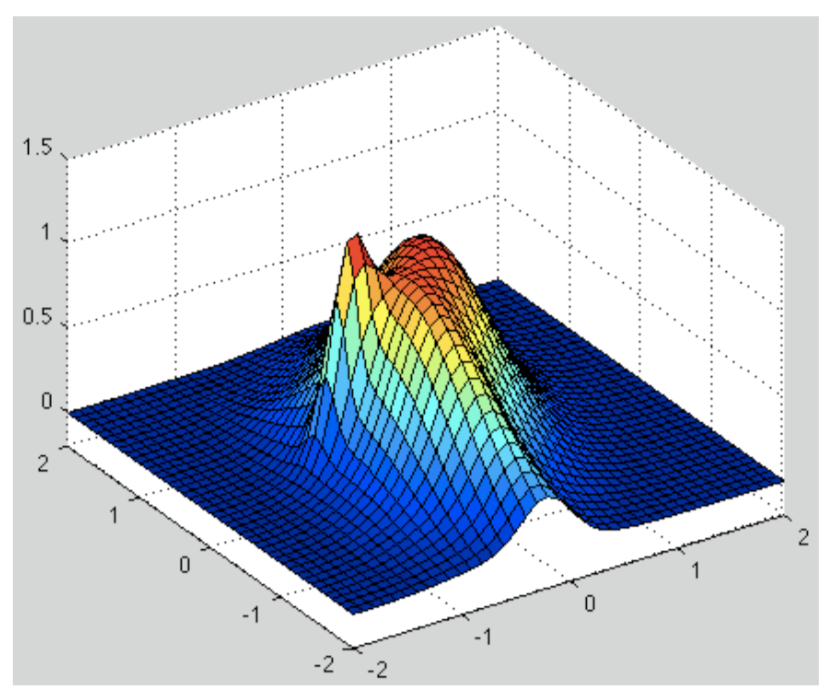
\includegraphics[width=0.4\textwidth]{Images/multi-modal.png}
\caption{Multi-modal probability density}
\label{Fig:multi-modal}
\end{figure}



After these preliminaries we are now going to train the network on the real data set.\\
Load the data using\\


\hspace{1cm} \texttt{data = load('a017\_NNpdfGaussMix.txt', '-ASCII');}

\hspace{1cm} \texttt{X = data(:,1:2); Y = data(:,3);}\\

\textbf{Answer:}\\






\subsection*{2.5}

Create a $2D$-plot of the target probability density function. Notice that the data is in the correct sequence to use in \texttt{surf()}.\\

\textbf{Answer:}\\








\subsection*{2.6}

Train the network on this data set. Use at least 40 hidden nodes and a learning rate parameter no higher than $\eta = 0.01$. Make sure the input data is properly randomized. Run the training phase for at least 2000 complete cycles and follow the progress by plotting the updated network output after every 20 full cycles. How does the final output of the network compare to the target distribution in the data? Explain. How could you improve the neural network in terms of speed of convergence and/or quality of the approximation?



\section*{Exercise 3 - Gaussian processes (weight 5)}


\textbf{Part 1 - Sampling from Gaussian stochastic processes}\\

One widely used kernel function for Gaussian process regression is given by the exponential of quadratic form, with the addition of constant and linear terms (eq. 6.63 Bishop):

\begin{eqnarray} \label{eq:5}
k(\textbf{x}, \textbf{x}') = \theta_0 \exp(- \frac{\theta_1}{2} || \textbf{x} - \textbf{x}' ||^2) + \theta_2 + \theta_3 \textbf{x}^T \textbf{x}'
\end{eqnarray}

We denote by $\boldsymbol{\theta}  = (\theta_0, \theta_1, \theta_2, \theta_3)$ the hyperparameter vector governing the kernel function $k$.

\subsection*{3.1.1}

Implement the kernel given by Equation (\ref{eq:5}) in Matlab as a function of $\textbf{x}, \textbf{x}'$ and $\boldsymbol{\theta}$. Note that $\textbf{x}$ can have any dimension.\\

\textbf{Answer:}\\





\subsection*{3.1.2}

We first consider the univariate case. For the parameter values $\boldsymbol{\theta} = (1,1,1,1)$ and $N = 101$ equally spaced points $\textbf{X}$ in the interval $[-1,1]$, compute the Gram matrix $\textbf{K(X,X)}$ (eq. 6.54 Bishop). What is the dimension of \textbf{K}? How can we show that \textbf{K} is positive semidefinite?\\

Note: Even when \textbf{K} is positive definitive, some of its eigenvalues may be too small to accurately compute (same for the determinant). This may pose a problem when generating a multivariate Gaussian distribution using \textbf{K} as its covariance matrix. You can alleviate this issue by adding a small diagonal term to \textbf{K}.\\


\textbf{Answer:}\\







\subsection*{3.1.3}

We will now use the previously computed matrix \textbf{K(X,X)} to produce samples from the Gaussian process prior $\textbf{y(X)} ~\mathcal{N}(\textbf{0, K(X,X)})$, with \textbf{X} being the previously determined N equally spaced points. Generate five functions \textbf{y(X)} with Matlab and plot them against the N input values \textbf{X}. Repeat the process (remember to compute a new \textbf{K} each time) for the hyperparameter configurations from Bishop, Figure 6.5:

\begin{align*}
\boldsymbol{\theta} \in \{(1,4,0,0),(9,4,0,0),(1,64,0,0),(1,0.25,0,0),(1,4,10,0),(1,4,0,5)\}.
\end{align*}

Describe the differences between the plots. Explain in which way each of the kernel parameters affects the generated samples.\\


\textbf{Answer:}\\





\subsection*{3.1.4}

We now move to the bivariate case. Instead of an interval, we now consider a 2-D grid of equally spaced points of size $N = 21 \times 21$ in $[-1,1] \times [-1,1]$. We collect all these grid points in a data matrix \textbf{X}, where each one of the 441 observations has two dimensions. What is the dimension of \textbf{K} now? What does this tell you about the scalability of sampling multivariate functions from Gaussian processes in higher dimensions?\\

\textbf{Answer:}\\






\subsection*{3.1.5}

Using the same kernel from (\ref{eq:5}), compute the Gram matrix \textbf{K(X,X)} on the grid for each hyperparameter configuration $\boldsymbol{\theta} \in \{(1, 1, 1, 1), (1, 10, 1, 1), (1, 1, 1, 10)\}$. For each \textbf{K}, generate and plot four random surfaces from the Gaussian process prior $\textbf{yX()} ~\mathcal{N}\textbf{(0, K(X,X)})$. Compare the observed differences to the univariate case.\\


\textbf{Answer:}\\








\textbf{Part 2 - Gaussian processes for regression}\\

We would like to apply Gaussian process models to the problem of regression (Bishop 6.4.2). We consider a noisy model of the form 

\begin{align*}
t_n = y_n + \epsilon_n,
\end{align*}

where $y_n = y(x_n)$ and $\epsilon_n$ are i.i.d. samples from a random noise variable on the observed target values. Furthermore, we assume that the noise process has a Gaussian distribution given by:

\begin{eqnarray} \label{eq:6}
p(t_n | y_n) = \mathcal{N}(t_n | y_n, \beta^{-1})
\end{eqnarray}

Going back to a one-dimensional input space, we consider the following training data consisting of four data points 

\begin{align*}
\mathcal{D} \{ (x_1 = -0.5, t_1 = 0.5), (x_2 = 0.2, t_2 = -1), (x_3 = 0.3, t_3 = 3),(x_4 = -0.1, t_4 = -2.5) \}
\end{align*}


\subsection*{3.2.1}

Just as before, compute the Gram matrix of the training data for $\boldsymbol{\theta} = (1,1,1,1)$. Then, taking $\beta = 1$ in Equation \ref{eq:6}, compute the covariance matrix \textbf{C} corresponding to the marginal distribution of the training target values: $p(\textbf{t}) = \mathcal{N}(\textbf{t} | \textbf{0, C})$.\\

\textbf{Answer:}\\






\subsection*{3.2.2}

Using the previous results, compute the mean and the covariance of the conditional distribution $p(t | \textbf{t})$ of a new target value $t$ corresponding to the input $x = 0$. Which equations from Bishop do you need?\\

\textbf{Answer:}\\







\subsection*{3.2.3}

Does the mean of the conditional distribution $p(t | \textbf{t})$ go to zero in the limit $x \to \pm \infty$? If so, explain why this happens. If not, how would you set the parameters $\boldsymbol{\theta}$ of the kernel function to make it happen?\\

\textbf{Answer:}\\

 


\section*{Exercise 4 - EM and doping (weight 5)}

In a certain hypothetical sport, banned substance '\textbf{X}' has become popular as a performance enhancing drug, as its presence is hard to establish in blood samples directly. Recently, it has been discovered that users of the drug tend to show a strong positive correlation between concentrations of two other quantities, $x_1$ and $x_2$, present in the blood. In contrast, 'clean' athletes tend to fall in one of two or three groups, that either show no or a negative correlation between $x_1$ and $x_2$. Unfortunately, as each sample contains only a single, instantaneous, measurement for each variable, it is not possible to establish this correlation from the sample. However, in many cases it is possible to distinguish to which \textit{class} a certain sample belongs by also looking at the values of two other measured variables, $x_3$ and $x_4$: certain combinations of measured values are often typical for one class but highly unusual for others.\\
After a high profile event, a large scale test has resulted in 2000 samples. Rumours suggest the number of positives could be as high as 20\%. However, the exact relationship between different classes and typical $x$ values is still not clear. This is where the EM-algorithm comes in...\\

The blood sample measurements are modelled as a mixture of $K$ Gaussians, one for each class

\begin{eqnarray} \label{eq:7}
p(x | \mu, \Sigma, \pi) = \sum^K_{k = 1} \pi_k \mathcal{N}(x | \mu_k, \sigma_k)
\end{eqnarray}

where $\textbf{x} = [x_1, x_2, x_3, x_4]$ represents the values for the measured quantities in the blood sample, $\mu = \{ \mu_1, ..., \mu_K\}$ and $\Sigma = \{ \Sigma_1, ..., \Sigma_K\}$ are the means and covariance matrices of the Gaussians for each class, and $\pi = \{ \pi_1, ..., \pi_K\}$ are the mixing coefficients in the overall data set.\\

Load the data using\\

\hspace{1cm} \texttt{data = load('a011\_mixdata.txt', '-ASCII');}\\

and set N to the number of datapoints and D to the number of variables in the dataset X.

\subsection*{4.1}

Try to give an estimate of the number, size and shape of the classes in the data, by plotting the distribution of the variables, e.g. using \texttt{hist()}, \texttt{scatter()} or \texttt{scatter3()}.\\

\textbf{Answer:}\\






\subsection*{4.2}

Implement an EM-algorithm using the description and formulas given in Bishop, §9.2.2. Use variable K for the number of classes and choose a priori equal mixing coefficients $\pi_k$. Initialize the means $\boldsymbol{\\mu}_k$, to random values around the sample mean of each variable, e.g. set $\mu_{k,1}$ to  $\bar{x}_1 + [-1 \leq \epsilon \leq +1]$. Initialize the $\Sigma_k$ to diagonal matrices with reasonably high variances, e.g. $4*\texttt{rand()}+2$, to avoid very small responsibilities in the first step. Make sure the EM-loop runs over at least 100 iterations. Display relevant quantities, at least the log likelihood (9.28), after each step so you can monitor progress and convergence. Write a plot routine that plots the $x_1, x_2$ coordinates of the data points, and color each data point according to the most probable component according to the mixture model.\\

\textbf{Answer:}\\






\subsection*{4.3}

Set $K = 2$, initialize your random generator and run the EM-algorithm on the data. Describe what happens. Try different random initializations and compare results.\\
\textit{(Should converge within 50 steps to two clusters, accounting for $\pm 1/3$ resp. $2/3$ of the data)}. Plot the $x_1, x_2$ coordinates colored according to the most probable component. Compute the correlation coefficients 

\begin{eqnarray} \label{eq:8}
p_{12} = \frac{cov[x_1, x_2]}{\sqrt{var[x_1] var[x_2]}}
\end{eqnarray}

of each of the components (i.e., use their covariance matrices to compute variances and covariances in (\ref{eq:8}), see also (Bishop, eq. (2.93))). Does either class show the characteristic strong\footnote{According to Wikipedia, the correlation is none if $|p| < 0.1$, small if $0.1 < |p| < 0.3$, medium if $0.3 < |p| < 0.5$ and strong if $|p| > 0.5$} positive correlation for $\{ x_1, x_2\}$?\\


\textbf{Answer:}\\







\subsection*{4.4}

Increase the number of classes to $K = 3$ and rerun your algorithm on the data, again trying different random initializations. Plot the $x_1, x_2$ coordinates colored according to the most probable component and compute the correlation coefficients of each of the components. Check both your plot and your coefficients if one of the clusters now displays the strong positive $\{ x_1, x_2\}$ correlation we are looking for.\\
Increase to $K = 4$, do the same, and see if this improves your result (in terms of detection of the doping-clusters). Based on your findings, is the rumoured 1-in-5 estimate for users of X credible?\\


\textbf{Answer:}\\



\subsection*{4.5}

Having found the offending cluster in the data using the EM-algorithm, we are now presented with four samples $\{ A, B, C, D\}$, with values for $[x_1, x_2, x_3, x_4]$ given as 

\begin{align*}
A &= [11.85, 2.2, 0.5, 4.0]\\
B &= [11.95, 3.1, 0.0, 1.0]\\
C &= [12.00, 2.5, 0.0, 2.0]\\
D &= [12.00, 3.0, 1.0, 6.3]
\end{align*}

One of these is from a subject who took drug X, and one is from a subject who tried to tamper with the test by artificially altering one or more of the $x_i$ levels in his/her blood sample.\\

Identify which sample belongs to the suspected user and which one belongs to the 'fraud'.\\

\textbf{Answer:}\\





\end{document}
